\documentclass[border=4pt]{standalone}
\usepackage{tikz}\usetikzlibrary{arrows.meta,positioning,calc}
\usepackage{amsmath}
\begin{document}
\sffamily\small
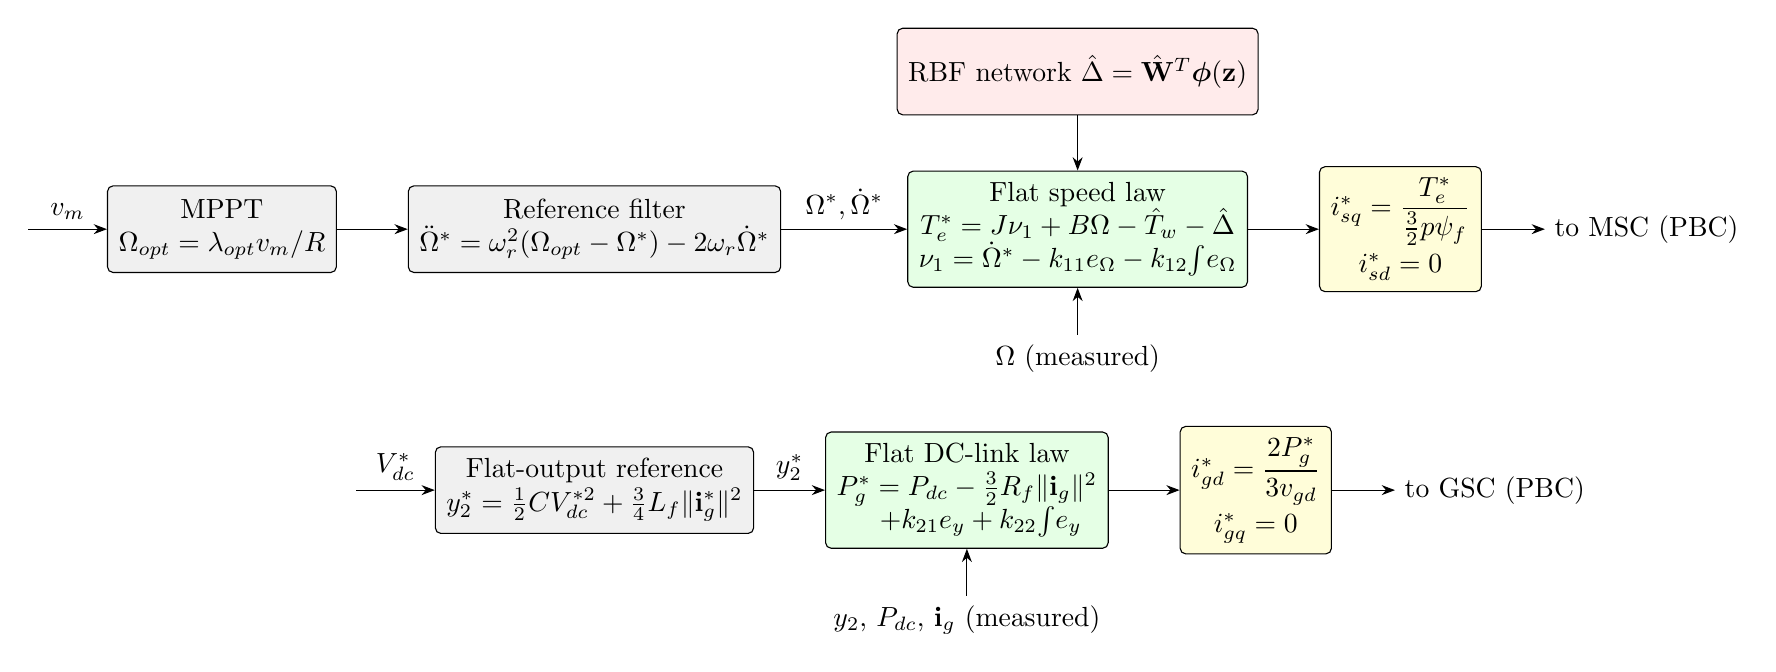
\begin{tikzpicture}[>=Stealth, node distance=6mm and 9mm,
  blk/.style={draw, rounded corners=2pt, minimum height=11mm, align=center, inner sep=4pt, fill=#1},
  blk/.default={blue!8}]
% speed channel
\node[blk=gray!12] (mppt) {MPPT\\$\Omega_{opt}=\lambda_{opt}v_m/R$};
\node[blk=gray!12, right=of mppt] (filt) {Reference filter\\$\ddot\Omega^*=\omega_r^2(\Omega_{opt}-\Omega^*)-2\omega_r\dot\Omega^*$};
\node[blk=green!10, right=16mm of filt] (fl1) {Flat speed law\\$T_e^*=J\nu_1+B\Omega-\hat T_w-\hat\Delta$\\$\nu_1=\dot\Omega^*-k_{11}e_\Omega-k_{12}\!\int\! e_\Omega$};
\node[blk=yellow!15, right=of fl1] (cur1) {$i_{sq}^*=\dfrac{T_e^*}{\frac32p\psi_f}$\\[2pt]$i_{sd}^*=0$};
\draw[->] ($(mppt.west)+(-10mm,0)$) -- node[above]{$v_m$} (mppt);
\draw[->] (mppt) -- (filt);
\draw[->] (filt) -- node[above]{$\Omega^*,\dot\Omega^*$} (fl1);
\draw[->] (fl1) -- (cur1);
\draw[->] (cur1.east) -- ++(8mm,0) node[right]{to MSC (PBC)};
\node[blk=red!8, above=7mm of fl1] (rbf) {RBF network $\hat\Delta=\hat{\mathbf W}^T\boldsymbol\phi(\mathbf z)$};
\draw[->] (rbf) -- (fl1);
\draw[<-] (fl1.south) -- ++(0,-6mm) node[below]{$\Omega$ (measured)};
% DC channel
\node[blk=gray!12, below=22mm of filt] (y2r) {Flat-output reference\\$y_2^*=\frac12CV_{dc}^{*2}+\frac34L_f\|\mathbf i_g^*\|^2$};
\node[blk=green!10, right=of y2r] (fl2) {Flat DC-link law\\$P_g^*=P_{dc}-\frac32R_f\|\mathbf i_g\|^2$\\$\quad+k_{21}e_y+k_{22}\!\int\! e_y$};
\node[blk=yellow!15, right=of fl2] (cur2) {$i_{gd}^*=\dfrac{2P_g^*}{3v_{gd}}$\\[2pt]$i_{gq}^*=0$};
\draw[->] ($(y2r.west)+(-10mm,0)$) -- node[above]{$V_{dc}^*$} (y2r);
\draw[->] (y2r) -- node[above]{$y_2^*$} (fl2);
\draw[->] (fl2) -- (cur2);
\draw[->] (cur2.east) -- ++(8mm,0) node[right]{to GSC (PBC)};
\draw[<-] (fl2.south) -- ++(0,-6mm) node[below]{$y_2$, $P_{dc}$, $\mathbf i_g$ (measured)};
\end{tikzpicture}
\end{document}
